\begin{figure}[h]
    \centering
    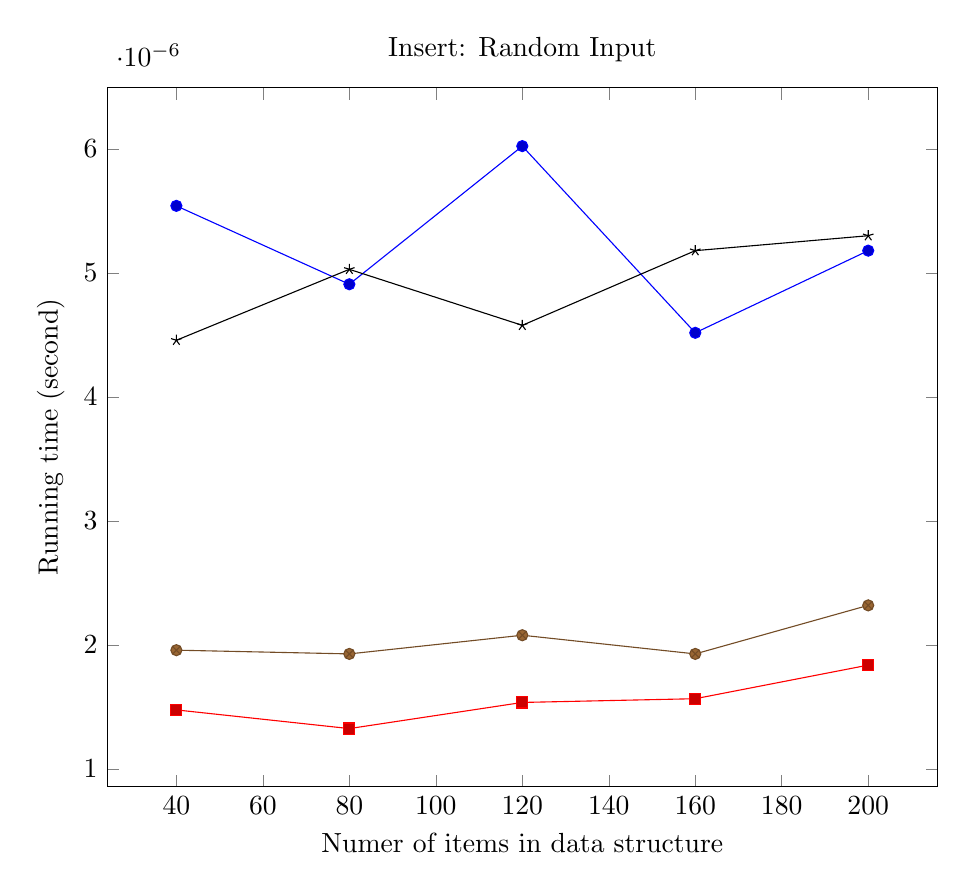
\begin{tikzpicture}
        \begin{axis}[
            xlabel={Numer of items in data structure},
            ylabel={Running time (second)},
            title={Insert: Random Input},
            width=\textwidth
        ]
		\addplot coordinates {
			(40, 5.541626196231553e-06)
			(80, 4.9091579890525596e-06)
			(120, 6.023506735033934e-06)
			(160, 4.517630051274757e-06)
			(200, 5.180215792129072e-06)
		};
		\addplot coordinates {
			(40, 1.4757591500824673e-06)
			(80, 1.3251714817072435e-06)
			(120, 1.5359942174344998e-06)
			(160, 1.5661117511098221e-06)
			(200, 1.8371695541849476e-06)
		};
		\addplot coordinates {
			(40, 1.9576396888862367e-06)
			(80, 1.9275221552109144e-06)
			(120, 2.0781098235861386e-06)
			(160, 1.9275221552109144e-06)
			(200, 2.3190500929873293e-06)
		};
		\addplot coordinates {
			(40, 4.4573949839255e-06)
			(80, 5.029628123753849e-06)
			(120, 4.577865118625401e-06)
			(160, 5.180215792127685e-06)
			(200, 5.300685926828974e-06)
		};
        \legend{}
        \end{axis}
    \end{tikzpicture}
    \caption{Average of 0 operations, benchmarked every 0, starting at 0.}
\end{figure}